% This text is proprietary.
% It's a part of presentation made by myself.
% It may not used commercial.
% The noncommercial use such as private and study is free
% Dec 2007
% Author: Sascha Frank 
% University Freiburg 
% www.informatik.uni-freiburg.de/~frank/
%
% 
\documentclass{beamer}
\setbeamertemplate{navigation symbols}{}

%\usetheme{Frankfurt}
\usetheme{Warsaw}

\usepackage[absolute,overlay]{textpos} 
\newenvironment{reference}[2]{% 
  \flushright\begin{textblock*}{\textwidth}(#1,#2) 
      \tiny\it\bgroup\color{gray!60!white}}{\egroup\end{textblock*}} 
\usepackage{listings}

\beamersetuncovermixins{\opaqueness<1>{25}}{\opaqueness<2->{15}}

\lstset{ %
language=Python,                % the language of the code
basicstyle=\tiny,               % the size of the fonts that are used for the code
numbers=left,                   % where to put the line-numbers
numberstyle=\tiny,              % the size of the fonts that are used for the line-numbers
stepnumber=2,                   % the step between two line-numbers. If it's 1, each line 
                                % will be numbered
numbersep=5pt,                  % how far the line-numbers are from the code
backgroundcolor=\color{white},  % choose the background color. You must add \usepackage{color}
showspaces=false,               % show spaces adding particular underscores
showstringspaces=false,         % underline spaces within strings
showtabs=false,                 % show tabs within strings adding particular underscores
frame=single,                   % adds a frame around the code
tabsize=2,                      % sets default tabsize to 2 spaces
captionpos=b,                   % sets the caption-position to bottom
breaklines=true,                % sets automatic line breaking
breakatwhitespace=false,        % sets if automatic breaks should only happen at whitespace
title=\lstname,                 % show the filename of files included with \lstinputlisting;
                                % also try caption instead of title
escapeinside={\%*}{*)},         % if you want to add a comment within your code
morekeywords={*,...}            % if you want to add more keywords to the set
}

\begin{document}
\title{Course Project}  
\author{Almost Finished}
\date{\today} 

\begin{frame}
\titlepage
\end{frame}

\begin{frame}
\frametitle{Table of contents}
\tableofcontents
\end{frame}

%data introduction
%spikes
%firing rates
%network introduction
%results

\section{Introduction} 
\subsection{Experimental Procedure}
\begin{frame}\frametitle{Experimental Procedure} 
   \begin{reference}{4mm}{85mm}
        Rickert J, Riehle A, Aertsen A, Rotter S, Nawrot MP (2009)
        Dynamic encoding of movement direction in motor cortical neurons
        Journal of Neuroscience 29: 13870-13882
   \end{reference}
 \begin{columns}
  \begin{column}{5cm}
   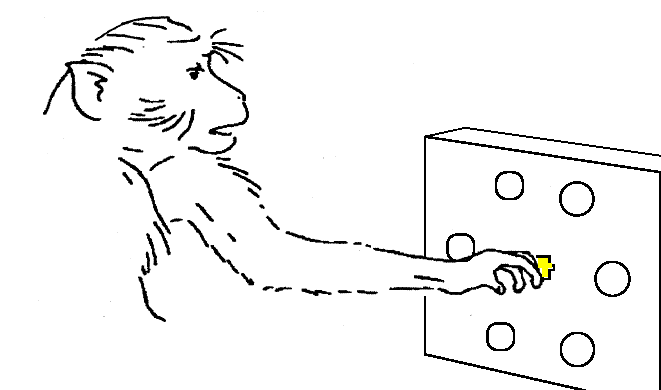
\includegraphics[scale=0.2]{fig/monkey.png}  
  \end{column}
  \begin{column}{5cm}
   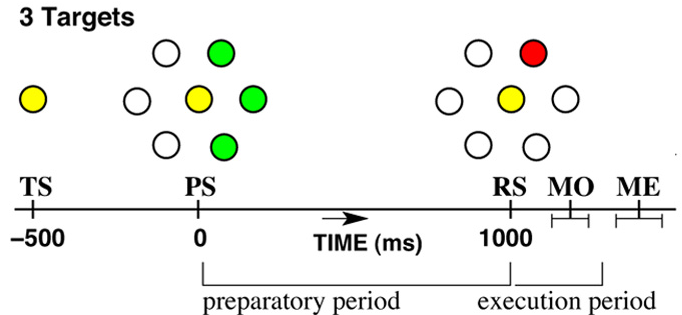
\includegraphics[scale=0.2]{fig/directions.png}  
  \end{column}
 \end{columns}
 \begin{itemize}
   \item Data by peak SNR
   \item Movement onset: $t_\rmmath{MO}=0$
   \item Time resolution: 1ms
  \end{itemize}
\end{frame}

\subsection{Approach}
\begin{frame}
 \begin{itemize}
  \item General discussion of neural network and synaptic weight update rule
  \item Splitting to two groups
  \begin{itemize}
    \item Group 1: Visualization of the data and the network output
    \item Group 2: Implementation of the neural network and weight update rules
  \end{itemize}
 \end{itemize}

\end{frame}

\section{Data Analysis}
\subsection{Spike Trains \& Firing Rates}
\begin{frame}\frametitle{Neuron 1}
\begin{columns}
 \begin{column}{5cm}
  \begin{figure}
   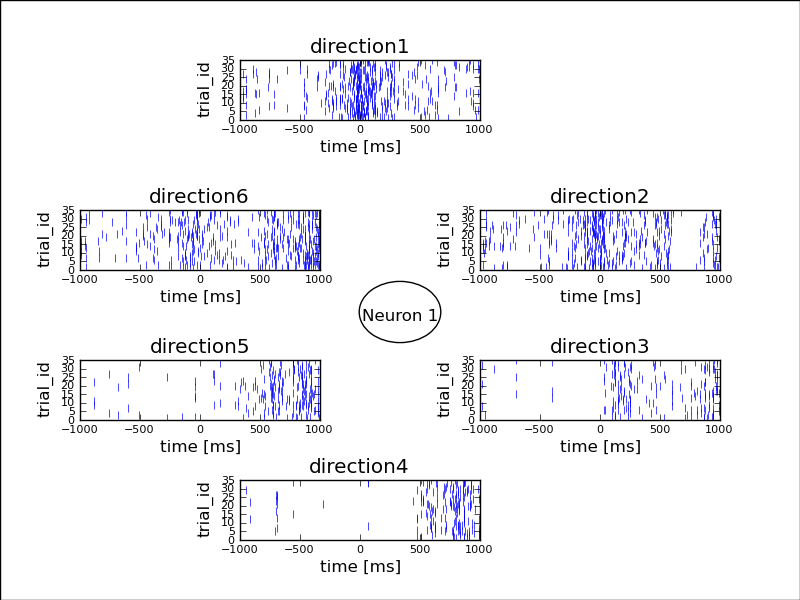
\includegraphics[scale=0.25]{fig/neuron1spikes.png}
   \caption{Spike trains against different trials}
  \end{figure}
 \end{column}
 \begin{column}{5cm}
  \begin{figure}
   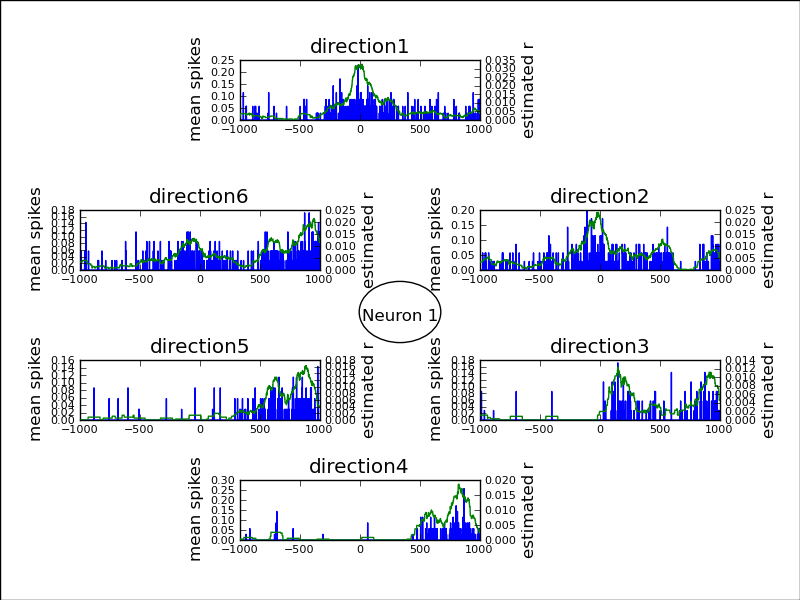
\includegraphics[scale=0.25]{fig/neuron1rates}
   \caption{Mean Number of Spikes \& Estimated Firing Rate}
  \end{figure}
 \end{column}
\end{columns}
\end{frame}
\begin{frame}\frametitle{Neuron 2}
\begin{columns}
 \begin{column}{5cm}
  \begin{figure}
   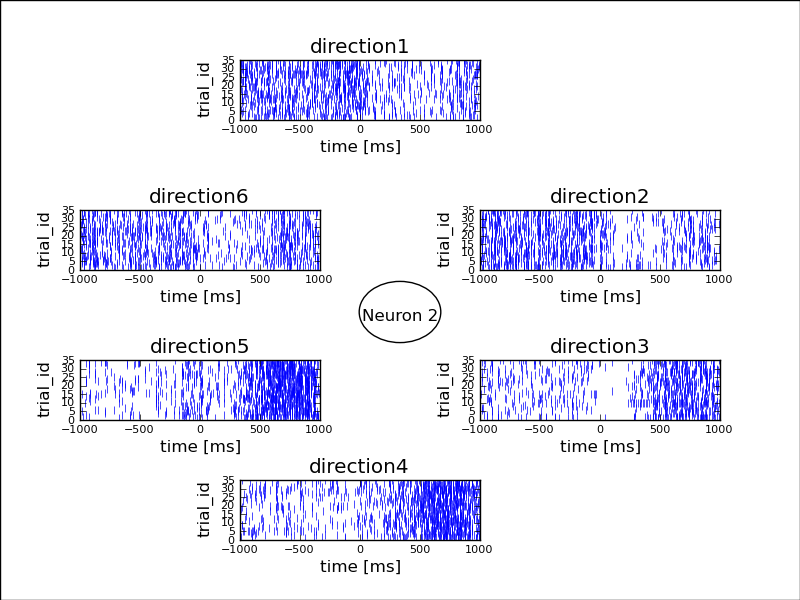
\includegraphics[scale=0.25]{fig/neuron2spikes.png}
   \caption{Spike trains against different trials}
  \end{figure}
 \end{column}
 \begin{column}{5cm}
  \begin{figure}
   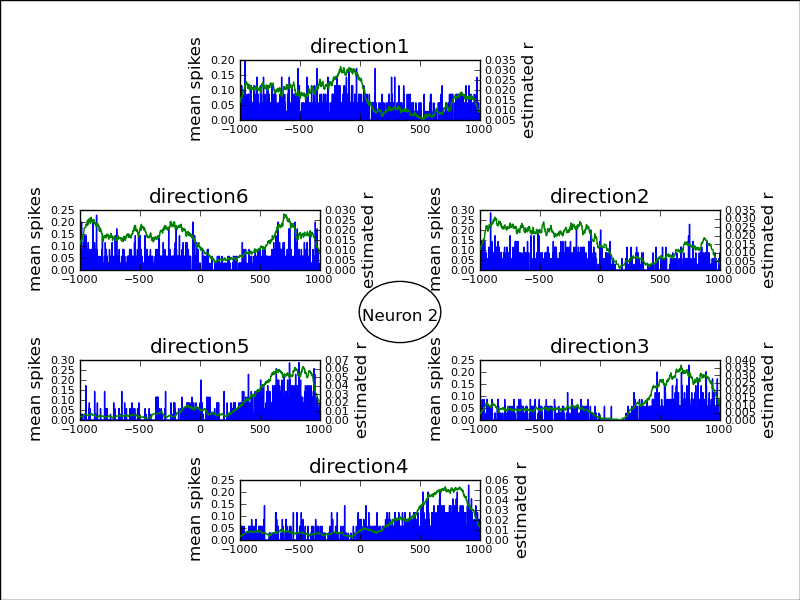
\includegraphics[scale=0.25]{fig/neuron2rates}
   \caption{Mean Number of Spikes \& Estimated Firing Rate}
  \end{figure}
 \end{column}
\end{columns}
\end{frame}

\begin{frame}\frametitle{Neuron 3}
\begin{columns}
 \begin{column}{5cm}
  \begin{figure}
   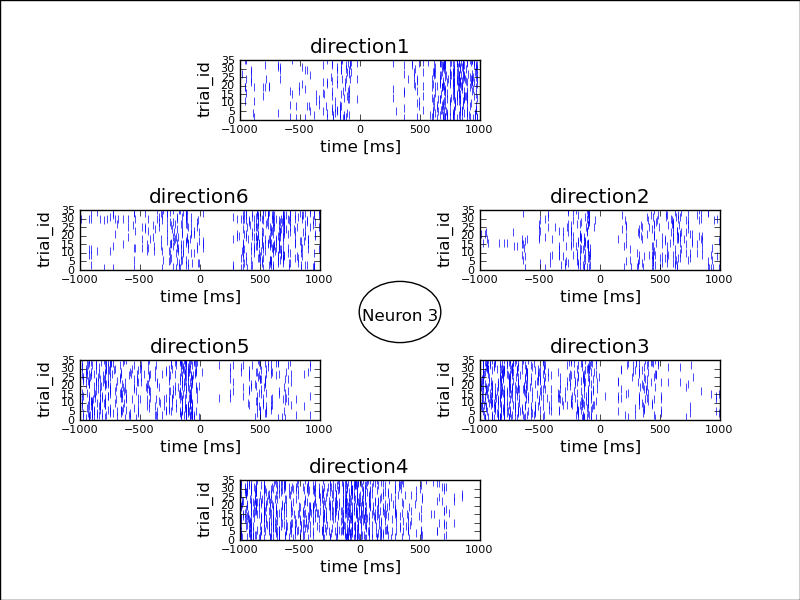
\includegraphics[scale=0.25]{fig/neuron3spikes.png}
   \caption{Spike trains against different trials}
  \end{figure}
 \end{column}
 \begin{column}{5cm}
  \begin{figure}
   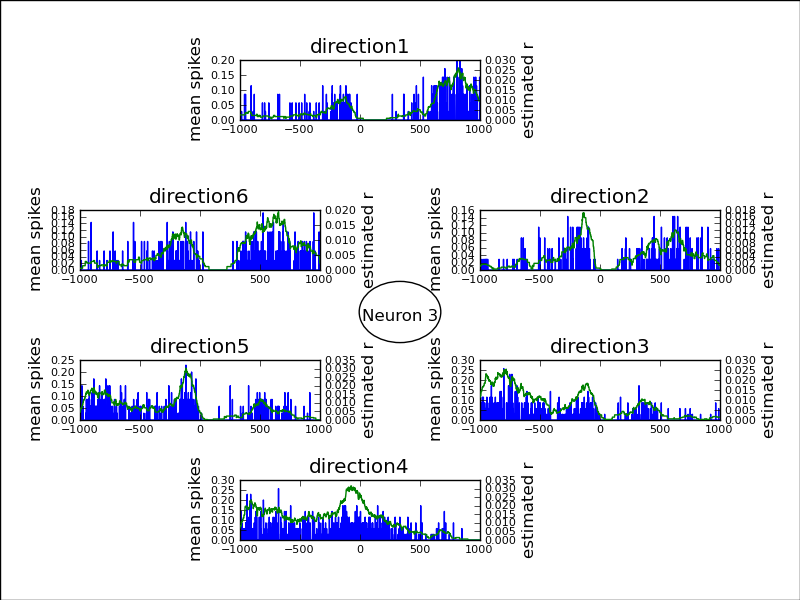
\includegraphics[scale=0.25]{fig/neuron3rates}
   \caption{Mean Number of Spikes \& Estimated Firing Rate}
  \end{figure}
 \end{column}
\end{columns}
\end{frame}

\begin{frame}\frametitle{Neuron 4}
\begin{columns}
 \begin{column}{5cm}
  \begin{figure}
   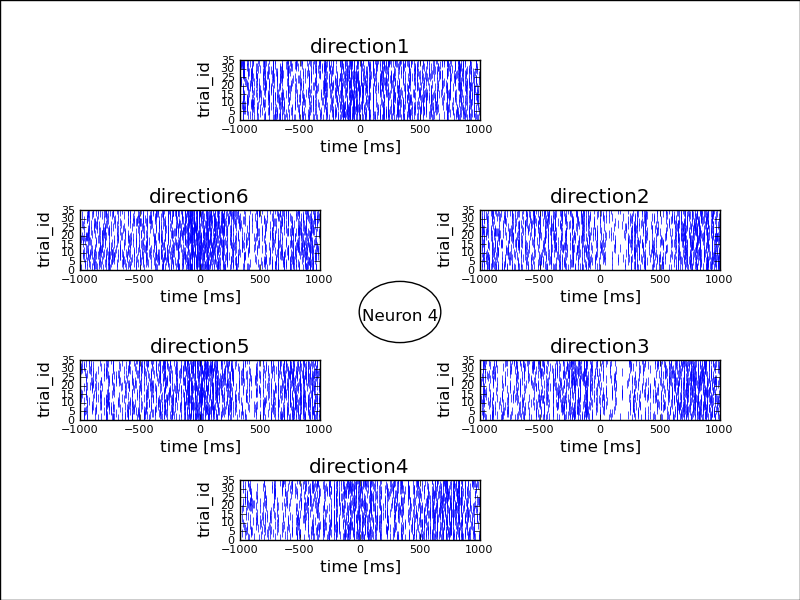
\includegraphics[scale=0.25]{fig/neuron4spikes.png}
   \caption{Spike trains against different trials}
  \end{figure}
 \end{column}
 \begin{column}{5cm}
  \begin{figure}
   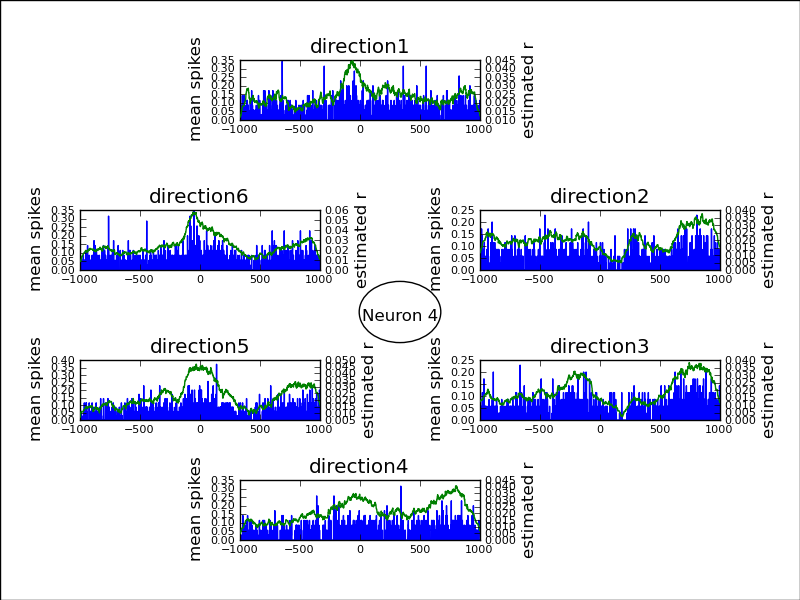
\includegraphics[scale=0.25]{fig/neuron4rates}
   \caption{Mean Number of Spikes \& Estimated Firing Rate}
  \end{figure}
 \end{column}
\end{columns}
\end{frame}

\begin{frame}\frametitle{Neuron 5}
\begin{columns}
 \begin{column}{5cm}
  \begin{figure}
   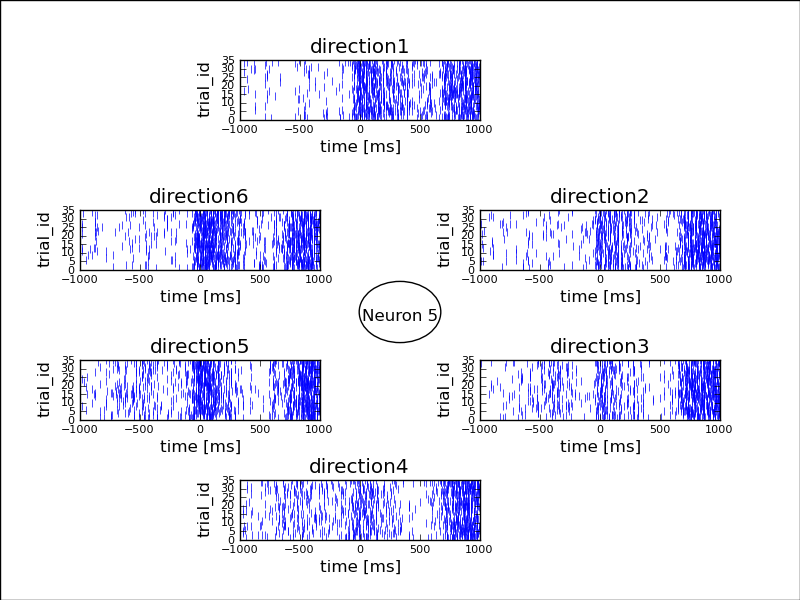
\includegraphics[scale=0.25]{fig/neuron5spikes.png}
   \caption{Spike trains against different trials}
  \end{figure}
 \end{column}
 \begin{column}{5cm}
  \begin{figure}
   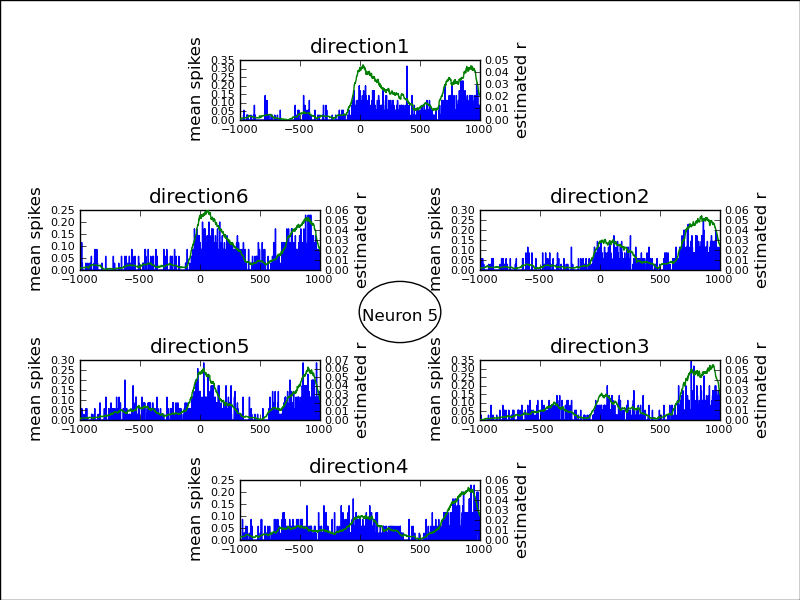
\includegraphics[scale=0.25]{fig/neuron5rates}
   \caption{Mean Number of Spikes \& Estimated Firing Rate}
  \end{figure}
 \end{column}
\end{columns}
\end{frame}

\section{Neural Network} 
\subsection{Realization}
\begin{frame}\frametitle{Realization of Neural Network}
\begin{figure}
   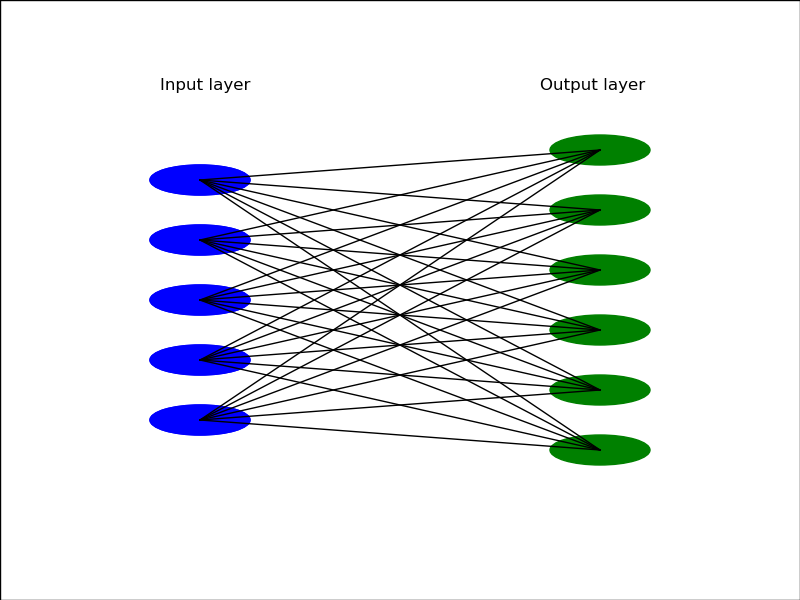
\includegraphics[scale=0.4]{fig/network}
   \caption{Network Description}
  \end{figure}
\end{frame}

% \subsection{Bayes' Rule}
% \begin{frame}\frametitle{Bayes' Rule}
%    \begin{reference}{4mm}{85mm}
%        Rickert J, Riehle A, Aertsen A, Rotter S, Nawrot MP (2009)
%        Dynamic encoding of movement direction in motor cortical neurons
%        Journal of Neuroscience 29: 13870-13882
%    \end{reference} 
% \begin{block}{Prediction of behavior from neural activity:}
% \begin{equation*}
%  P(d|r) = P(d|r) \cdot \frac{P(d)}{P(r)}
% \end{equation*}
% \end{block}
% \begin{eqnarray*}
%  d &=& \text{Movement Direction} \\
%  r &=& \text{Firing Rate} \\
%  P(d) &=& \text{Directional tuning profile} \\
%  P(r) &=& \text{\emph{prediction} of direction from rate}
% \end{eqnarray*}
% \end{frame}

\subsection{Python Code}
\begin{frame}[fragile]
    \frametitle{Python code: update rule}
%\pause
 \begin{lstlisting}
for every trial:

    for every direction:

        - run the network
        - determine active synapses
        - update the weights:
            if the prediction was correct:
              - increase the active synapses
              - decrease the inactive synapses
            else:
              - decrease the active synapses
              - increase the inactive synpases



active synapses: higher firing rate than their average firing rate

 \end{lstlisting}

% for input_id, weight in enumerate(weight_list):
%     firing_rate = input_firing_rates[input_id]
%     value = firing_rate - average_firing_rates[input_id]
%     #value += 2
%     if value > 0:
%        if id == highest_output_index:
%            for syn_id, synapse in enumerate(weight):
%                if syn_id == highest_output_index:
%                     newWeight = weight[syn_id] + value * maxchange
%                else:
%                     newWeight = weight[syn_id] - 0.1 * value * maxchange
%                if newWeight > 0.001 and newWeight < 1.:
%                     weight[syn_id] = newWeight
\end{frame} 

\subsection{Results}

\begin{frame}
 
  %\begin{figure}
  Demonstration...
  %\includegraphics[scale=0.5]{fig/test_network_trial??_direction?.png} 
  %\caption{}
 %\end{figure}
\end{frame}


\section{Closure}
\begin{frame}[plain]
 \frametitle{Closure}
 \begin{figure}
  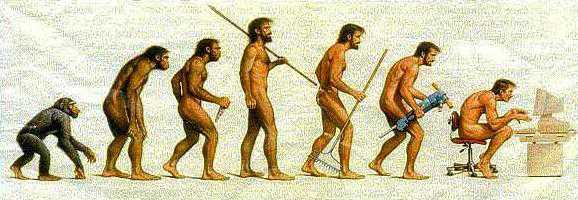
\includegraphics[scale=0.5]{fig/Evolution.jpg} 
  \caption{Last Day of Lecture}
 \end{figure}
\end{frame}

\end{document}